\section{Exercise 3}

The standardization procedure ensures that the random samples from a normal distribution maintain a mean of 0 and a variance of 1, aligning with the theoretical assumptions of the Black-Scholes model.

The Black-Scholes model assumes that stock prices follow a geometric Brownian motion, requiring normally distributed random variables with specific statistical properties. In the simulation, stock price paths are generated according to
\begin{equation}
    S_{t+\Delta t} = S_t \exp\left((r - \frac{1}{2}\sigma^2)\Delta t + \sigma\sqrt{\Delta t}Z\right),
\end{equation}
where $Z \sim N(0,1)$ represents standard normal random variables. In practice, computer-generated random numbers may not perfectly maintain these statistical properties, particularly with smaller sample sizes.

The analytical price of a European call option is computed using the Black-Scholes formula:
\begin{equation}
    C = S_0 \Phi(d_1) - K e^{-rT} \Phi(d_2),
\end{equation}
where
\begin{equation}
    d_1 = \frac{\ln(S_0 / K) + (r + \frac{1}{2} \sigma^2)T}{\sigma \sqrt{T}}, \quad d_2 = d_1 - \sigma \sqrt{T}.
\end{equation}
Here, $\Phi(\cdot)$ represents the cumulative distribution function of the standard normal distribution.

A Monte Carlo simulation is implemented to price a European call option using the following parameters:

\begin{center}
    \begin{tabular}{l c c}
        \toprule
        Parameter & Symbol & Value \\
        \midrule
        Initial Stock Price & $S_0$ & 100.0 \\
        Strike Price & $K$ & 95.0 \\
        Risk-free Rate & $r$ & 0.03 \\
        Volatility & $\sigma$ & 0.10 \\
        Time to Maturity & $T$ & 1.0 \\
        \bottomrule
    \end{tabular}
\end{center}

The analytical solution using the Black-Scholes formula yields a price of $8.934954$. Two versions of the Monte Carlo simulation were compared: one using standardized random samples to ensure a mean of 0 and standard deviation of 1, and another using raw random samples directly. The convergence is tested by varying the number of simulation paths from 2 to 10000. \\

\vspace{0.25cm}

\begin{figure}[h!]
\centering
\begin{minipage}{0.5\textwidth}
    \centering
    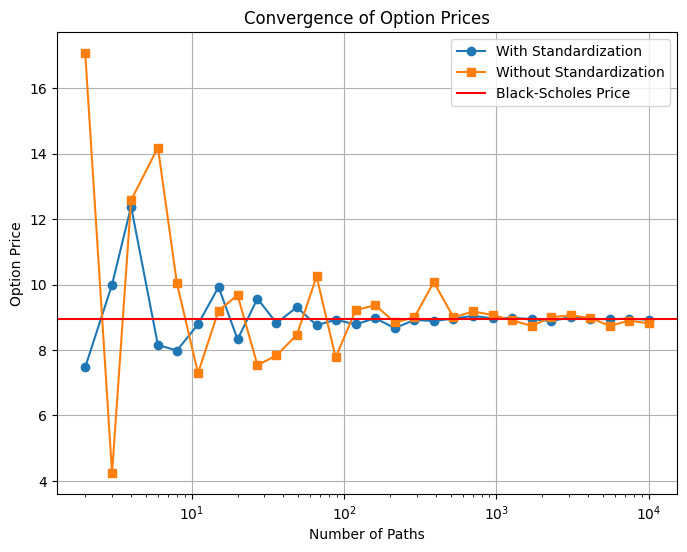
\includegraphics[width=0.95\textwidth]{Exercise_set_01/img/ConvergenceStdVsNon.png}\\
    \caption{Convergence of option price estimates with and without standardization}
    \label{fig:StdVsNonConv}
\end{minipage}%
\begin{minipage}{0.5\textwidth}
    \centering
    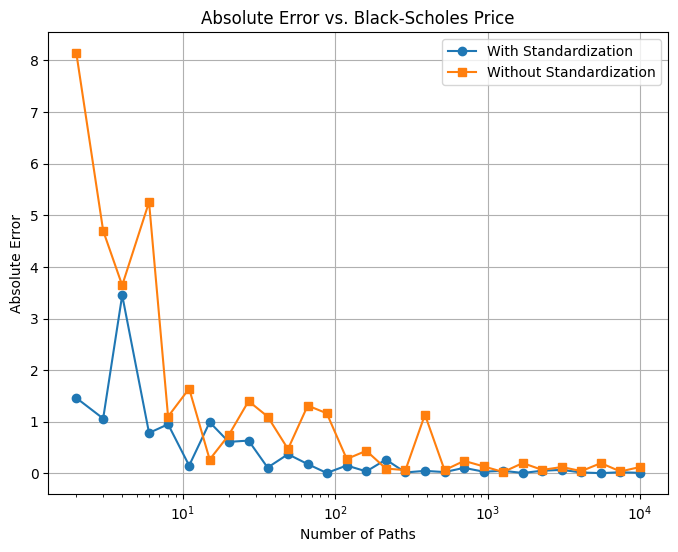
\includegraphics[width=0.95\textwidth]{Exercise_set_01/img/ConvergenceAbsValue.png}\\
    \caption{Absolute error in option price estimates with and without standardization}
    \label{fig:StdVsNonAbs}
\end{minipage}
\end{figure}

\vspace{0.5cm}

Figures \ref{fig:StdVsNonConv} and \ref{fig:StdVsNonAbs} illustrate the effect of standardization on the convergence and accuracy of Monte Carlo option price estimates. The standardized method exhibits greater stability, especially when the number of simulation paths is small, leading to a smoother and more consistent convergence toward the analytical Black-Scholes price.\\
In contrast, the non-standardized approach shows significant fluctuations at lower path counts, with price estimates displaying considerable variability. The absolute error plot further highlights the advantage of standardization, as it consistently results in lower errors across different path counts. The non-standardized approach, on the other hand, produces substantially larger errors, particularly when the number of paths is below 100, demonstrating its inefficiency in scenarios with limited simulations. \\

In addition to this, stability analysis is performed using 1000 different random seeds with a fixed path count of 100.\\

\begin{figure}[h!]
\centering
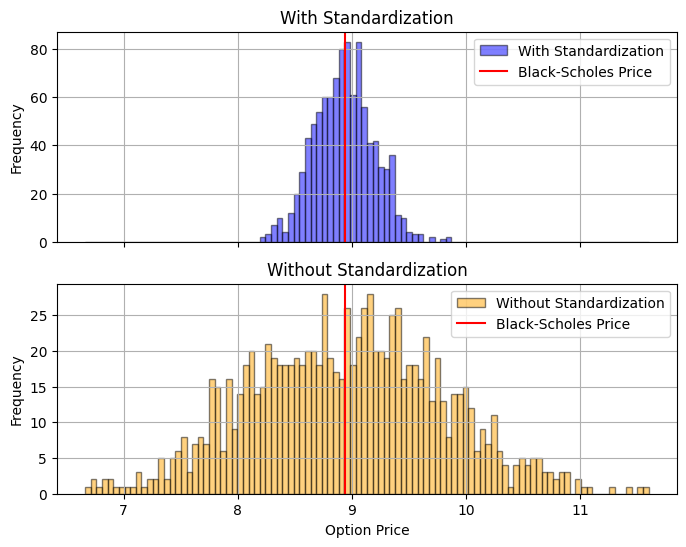
\includegraphics[width=0.5\textwidth]{Exercise_set_01/img/DistStdVsNon.png} \
\caption{Standardization vs without standardization option price estimation}
\label{fig:distStdVsNon}
\end{figure}

\begin{center}
\begin{tabular}{l c c c}
\toprule
Method & Mean Price & Standard Deviation & Mean Absolute Error \\
\midrule
With Standardization & 8.933259 & 0.260974 & 0.208185 \\
Without Standardization & 8.951233 & 0.845786 & 0.686860 \\
Black-Scholes (Analytical) & 8.934954 & - & - \\
\bottomrule
\end{tabular}
\end{center}

The distribution of option prices from simulations with 1000 different random seeds is presented in Figure (\ref{fig:distStdVsNon}). The standardized method produces a tighter, more normally distributed set of prices centered closely around the analytical Black-Scholes price. The non-standardized method yields a wider, more irregular distribution with greater variance. Furthermore, one observes that with standardization, the mean price of 8.933259 closely approximates the analytical Black-Scholes price of 8.934954, with a standard deviation of merely 0.260974. In contrast, the non-standardized approach yields a mean price of 8.951233 with a substantially higher standard deviation of 0.845786. The mean absolute error confirms this superior performance, with the standardized method achieving 0.208185 compared to 0.686860 for the non-standardized approach. \\

The standardization process effectively functions as a variance reduction technique, producing more consistent results with fewer simulation paths. This effect is evident in the significantly lower standard deviation of the standardized method compared to the non-standardized approach. By enforcing the theoretical properties of normal random variables with mean 0 and variance 1, one ensures that the simulation adheres more closely to the theoretical model's assumptions, thereby enhancing the accuracy and reliability of the option pricing estimates. The improved statistical precision consequently leads to faster convergence, requiring fewer paths to achieve comparable accuracy to the analytical solution. \\

To sum up, standardizing random samples in Monte Carlo simulations for option pricing under the Black-Scholes model provides significant benefits in terms of accuracy, efficiency, and reliability. The standardized approach converges faster to the analytical solution, exhibits lower variability across different random seeds, and produces consistently lower errors compared to the non-standardized method.
